\documentclass[25pt]{sciposter}

\usepackage[T1]{fontenc}
\usepackage[utf8]{inputenc}

\usepackage{amsthm}

\usepackage[dvipsnames,usenames,svgnames,table]{xcolor} 
\usepackage{lipsum}
\usepackage{epsfig}
\usepackage{amsmath}
\usepackage{amssymb}
\usepackage[german]{babel}
\usepackage{geometry}
\usepackage{multicol}
\usepackage{graphicx}
\usepackage{tikz}
\usepackage{wrapfig}
\usepackage{gensymb}
\usepackage[utf8]{inputenc}
\usepackage{empheq}

\usepackage{pgfplots}
\pgfplotsset{width=11cm,compat=1.9}


% for nice tableas
\usepackage{booktabs}

\graphicspath{ {img/} }

\geometry{
 landscape,
 a1paper,
 left=5mm,
 right=50mm,
 top=5mm,
 bottom=50mm,
 }
\usepackage{array}   % for \newcolumntype macro
\newcolumntype{L}{>{$}m{5.5cm}<{$}} % math-mode version of "l" column type

%BEGIN LISTINGDEF





\newcommand*\widefbox[1]{\fbox{\hspace{2em}#1\hspace{2em}}}
\newcommand{\limm}{\lim\limits_{n \to \infty}}
\newcommand{\limx}[1]{\lim\limits_{x \to #1}}
\newlength\dlf  % Define a new measure, dlf
\newcommand\alignedbox[2]{
% Argument #1 = before & if there were no box (lhs)
% Argument #2 = after & if there were no box (rhs)
&  % Alignment sign of the line
{
\settowidth\dlf{$\displaystyle #1$}
    % The width of \dlf is the width of the lhs, with a displaystyle font
\addtolength\dlf{\fboxsep+\fboxrule}
    % Add to it the distance to the box, and the width of the line of the box
\hspace{-\dlf}
    % Move everything dlf units to the left, so that & #1 #2 is aligned under #1 & #2
\boxed{#1 #2}
    % Put a box around lhs and rhs
}
}
\usepackage{graphicx,url}

%BEGIN TITLE
\title{\huge{Analysis 2}}

\author{\large{David Zollikofer}}
%END TITLE

\usepackage{palatino}
\usepackage{eulervm}
% begin custom commands
\newcommand{\Q}{\mathbb{Q}}
\newcommand{\R}{\mathbb{R}}
\newcommand{\N}{\mathbb{N}}
%\newcommand{\cos}{\operatorname{cos}}
%\newcommand{\sin}{\operatorname{sin}}
%\newcommand{\exp}{\operatorname{exp}}

\newtheorem{thm}{Thm}[section]

\newcommand{\norm}[1]{\left\lVert#1\right\rVert}
\usepackage[framemethod=TikZ]{mdframed}
\newenvironment{method}[1]{\begin{mdframed}[backgroundcolor=blue!10,innertopmargin=15pt, innerbottommargin=15pt, nobreak=true]
		\textbf{#1 }
	}
	{ 
	\end{mdframed}
}

\newenvironment{important}{\begin{mdframed}[backgroundcolor=red!50,innertopmargin=15pt, innerbottommargin=15pt, nobreak=true]
		\Large
	}
	{ 
	\end{mdframed}
}

\newenvironment{lemma}{\begin{mdframed}[backgroundcolor=gray!50,innertopmargin=15pt, innerbottommargin=15pt, nobreak=true]
		\Large
	}
	{ 
	\end{mdframed}
}



\usepackage{todonotes}
\newcommand{\TODO}[1]{\todo[inline]{\Large TODO:  #1}}


\usepackage{mathpazo}


\DeclarePairedDelimiter\abs{\left|}{\right|}%



\setlength\abovedisplayskip{0pt}

\renewcommand{\familydefault}{\rmdefault}

% end custom commands

\begin{document}





\maketitle


\begin{multicols}{3}



\section{Einführung}


\subsection*{Wichtige Ungleichungen}

\begin{method}{Bernoulli Ungleichung}
	Wenn $x\in \R$ mit $x > -1$ sowie $n \in \mathbb{Z}$ mit $n >0$, dann gilt:
	\begin{align*}
		\left(1 + x\right) ^n \geq 1 + nx
	\end{align*}
	\textit{Beweis:} per Induktion
\end{method}


\begin{method}{Cauchy Schwarz}
	$\forall x,y\in \R^n$ gilt $|\langle x,y\rangle| \leq ||x||\cdot||y||$.
\end{method}


\begin{method}{Komplexe Zahlen} ${\displaystyle \varphi =\arg(z)}$\\
\begin{empheq}[box=\fbox]{align*}
	z &= x + iy & z &= r(\cos(\phi) + i\sin(\phi)) & z &= re^{i\phi}
\end{empheq}
\begin{empheq}[box=\fbox]{align*}
x &= r \cos \phi &  y &= r\sin \phi & r &= \sqrt{x^2 + y^2} & \phi &= \arctan\left(\frac{x}{y}\right) 
\end{empheq}
\textsc{Division:} Es gilt $z^{-1} = \frac{\bar{z}}{||z||^2}$ wenn $z \not = 0$\\
\textsc{Polarform} Wenn \begin{align*}
z_1 &= r_1(\cos(\theta_1) + i\sin(\theta_1))\\
z_2 &= r_2(\cos(\theta_2) + i\sin(\theta_2))
\end{align*}
dann gilt: 
\begin{align*}
z_1 \cdot z_2 &= r_1 \cdot r_2 \left(\cos(\theta_1 + \theta_2) + i\sin(\theta_1 + \theta_2)\right)\\
\frac{z_1}{z_2} &= \frac{r_1}{r_2}\left(\cos(\theta_1 - \theta_2) + i\sin(\theta_1 - \theta_2)\right)
\end{align*}
Zudem folgt durch Induktion:
\begin{align*}
	z^n = r^n (\cos(n\theta) + i \sin(n \theta))
\end{align*}

\textbf{Komplexe Nullstellen:} Die $n$-te Wurzel von $x$ berechnen wir (es gibt $n$ davon):
\begin{align*}
	\sqrt[n]{z} &= \sqrt[n]{r} e^{i \left( \frac{\phi_0}{n} + \frac{2k\pi}{n}\right)}\\
	&= \sqrt[n]{r} \left(\cos\left( \frac{\phi_0}{n} + \frac{2k\pi}{n}\right) + i \sin\left( \frac{\phi_0}{n} + \frac{2k\pi}{n}\right)\right)
\end{align*}

\end{method}




% -------------------------- Grenzwerte --------------------------

\section*{Grenzwerte}
Wir sagen dass $f$ an der Stelle $a$ den Grenzwert $L\in \R$ hat, geschrieben $\lim\limits_{x \to a} f(x) = L$ falls $\forall \epsilon > 0 \ \exists \delta > 0 $ sodass für alle $|x-a|<\delta$ gilt $|f(x)-L|< \epsilon$


\begin{method}{Grenzwert mittels Dominanz}
Grundsätzlich gelten die folgenden Dominanzen: \\
Für $x \to + \infty$:
\begin{align*}
	\ldots < \log(\log(x)) < \log(x) < x^\alpha < e^x < \alpha^x < x! < x^x
\end{align*}
Sowie für $x \to 0^+$
\begin{align*}
\ldots < \log(\log(x)) < \log(x) < \left(\frac{1}{x}\right)^\alpha
\end{align*}
\end{method}


\subsubsection*{Wurzeltrick}
\begin{align*}
	\lim\limits_{x \to \infty } \left( \sqrt{x^2 + x} -x \right) &= \lim\limits_{x \to \infty } \left( \sqrt{x^2 + x} -x \right)  \cdot \frac{  -\sqrt{x^2 + x} -x  }{ -\sqrt{x^2 + x} -x }\\
	&= 	\lim\limits_{x \to \infty } \frac{- \sqrt{x^2 + x} ^2 + x^2}{ -\sqrt{x^2 + x} -x}\\
	&= 	\lim\limits_{x \to \infty } \frac{x^2 + x - x^2}{ \sqrt{x^2 + x} +x}\\
	&=  \lim\limits_{x \to \infty}  \frac{1}{\sqrt{1 + \frac{1}{x}} + 1} = \frac{1}{2}
\end{align*}



\begin{method}{Fundamentallimes}
	Oft kann man einen dieser Limits verwenden:
	\begin{align*}
		\lim\limits_{x \to \infty} \left(1 + \frac{1}{x}\right)^x &= e &  \lim\limits_{x \to 0} \frac{\sin(x)}{x} &= 1 \\
		\lim\limits_{n \to \infty} \frac{a^n}{n^n} &= 0 & 	\lim\limits_{n \to \infty} \sqrt[n]{n} &= 1\\
		\lim\limits_{n \to \infty} \sqrt[n]{a} &= 1  & 	\lim\limits_{n \to \infty} \frac{1}{\sqrt[n]{n!}} &= 0
	\end{align*}
\end{method}


\begin{method}{Variablenwechsel für Grenzwert}
	Seien $f,g$ Funktionen wobei $f$ stetig in $y_0$ und $g$ stetig in $x_0$ mit $y_0 = \lim\limits_{x \to x_0} g(x)$ ist. Dann gilt:
	\begin{align*}
		\lim_{(x\to x_0)}f(g(x)) = \lim_{(y\to y_0)} f(y)
	\end{align*}
\end{method}

\begin{method}{Bernoulli - de l’Hospital}
	Wenn wir zwei differenzierbare Funktionen $f$, $g$ haben mit $g'(a)\not = 0$ dann gilt falls:
	\begin{itemize}
		\item entweder $\lim_{x \to a} f(x) = \lim_{x \to a} g(x) = 0 $
		\item oder $\lim_{x \to a} f(x) = \lim_{x \to a} g(x) = \infty $
	\end{itemize}
	dann gilt:
	\begin{equation*}
	\lim_{x \to a} \frac{f(x)}{g(x)} = 	\lim_{x \to a} \frac{f'(x)}{g'(x)}
	\end{equation*}
\end{method}
\begin{itemize}
	\item \textbf{Typ 1: $\frac{0}{0}$ oder $\frac{\infty}{\infty}$}\\
	
	\item \textbf{Typ 2: $0 \cdot \infty$} Wenn wir einen Grenzwert wie $\lim\limits_{x \to a} f(x)g(x)$ haben dann können wir den umformen in:
	\begin{align*}
	\lim_{x \to a}f(x) g(x) &= \lim_{x\to a} \frac{f(x)}{\frac{1}{g(x)}}\\
	\lim_{x \to a}f(x) g(x) &= \lim_{x\to a} \frac{g(x)}{\frac{1}{f(x)}}
	\end{align*}

	
	
	\item \textbf{Typ 3: $f(x)^{g(x)}$} Wenn wir Grenzwerte des Types $ \limx{a} f(x)^{g(x)}$ haben, dann schreiben wir es wie folgt:
	\begin{align*}
	\limx{a} f(x)^{g(x)} &= \limx{a} e^{\ln(f(x))\cdot g(x)} = e^{\limx{a} \ln(f(x))\cdot g(x)}
	\end{align*}

\end{itemize}

\subsection*{Taylor (als letzte Hoffung)}
Wenn das alles nicht funktioniert kann man versuchen die Taylorentwicklung einzusetzten. \\

\begin{important}
Kann auch sinnvoll sein Audruck wie $\sqrt{x} = t$ zu subsituieren und dann neuer Limes.
\end{important}



% -------------------------- Folgen --------------------------

\section*{Folgen}

\begin{method}{Definition Konvergenz}
Folge $a_n$ is konvergent, falls $\exists l \in \mathbb{R}$ so dass $\forall \epsilon > 0$ die Menge $\{n \in \mathbb{N}^+: a_n \not \in (l-\epsilon, l + \epsilon)\}$ endlich ist. \\
Äquivalent: $\forall \epsilon > 0 \ \exists N \in \N $ so dass $ \forall n \geq N$ gilt $|a_n - l|< \epsilon$.
\end{method}

\textbf{Beispiel (Konvergenz mit Definition)}: 
Beweise dass $\limm \frac{3n^2 + 4}{2n^2 + 1} = \frac{3}{2}$. Sei $\epsilon > 0$. Dann muss gelten $|a_n - a | < \epsilon$. Somit $\left| \frac{3n^2 + 4}{2n^2 + 1} -  \frac{3}{2}\right| = \left| \frac{6n^2 + 8 - 6n^2 -3}{4n^2 + 2} \right| = \frac{5}{4n^2 + 2} < \epsilon$. Gibt $4n^2 + 2 > \frac{5}{\epsilon}$, äquiv zu $n > \sqrt{\frac{5}{4 \epsilon} - \frac{1}{2}}$. Wir definieren $N = \lfloor \sqrt{\frac{5}{4 \epsilon} - \frac{1}{2}} \rfloor$. Nun gilt $\forall n \geq N : |a_n - a | < \epsilon$.




\begin{method}{Rechnen mit Grenzwerten} $(a_n)_n$ und $(b_n)_n$ konvergent mit GW $a,b$. Dann gilt:
	\begin{itemize}
		\item $\lim \limits_{n \to \infty} (a_n + b_n) = a + b$	
		\item $\lim \limits_{n \to \infty} (a_n \cdot b_n) = a \cdot b$
		\item  Falls $b_n, b \not = 0$, so gilt $\lim \limits_{n \to \infty} \frac{a_n}{b_n} = \frac{a}{b}$
		\item Falls $a_n \leq b_n$ $\forall n \in \mathbb{N}$, so gilt $a \leq b$
	\end{itemize}
\end{method}

\textbf{Beispiel (Rechnen mit Grenzwerten)}: 
\begin{itemize}
	\item $\limm  \frac{(\frac{1}{n} + n^2 )^3}{1 + n^6} = \limm \frac{n^6}{n^6} \frac{(\frac{1}{n^3} + 1 )^3}{\frac{1}{n^6} + 1} = \limm \frac{(\frac{1}{n^3} + 1 )^3}{\frac{1}{n^6} + 1} = 1$
	
	\item $\limm \sqrt{n} (\sqrt{n + 2} - \sqrt{n}) \stackrel{\text{Wurzeltrick}}{=} \limm \frac{2 \sqrt{2}}{\sqrt{n+2} + \sqrt{n}} = \limm  \frac{2}{\sqrt{1 + \frac{2}{n}} + 1} = 1$
	
	\item $ \limm \sqrt[n]{3^n + 7^n} = \limm \sqrt[n]{7^n ( \frac{3^n}{7^n} + 1)} = \limm 7 \sqrt[n]{ (\frac{3^n}{7^n} + 1)} = 7$
	
\end{itemize}


\begin{method}{Sandwich Theorem}
Seien $b_n \leq a_n \leq c_n$. Falls $b_n$ und $c_n$ konvergent sind mit $\lim \limits_{n \to \infty } b_n = \lim \limits_{n \to \infty } c_n = L$, so ist $a_n$ auch konv. mit $\lim \limits_{n \to \infty } a_n = L$
\end{method}
\textbf{Beweis (Sandwich Theorem)}: 
Da $b_n$, $c_n$ konvergent mit GW $L$:
$$\forall \epsilon > 0 \exists N_1 : \forall n \geq N_1 : L-\epsilon < b_n + \epsilon$$
Analog  $ \exists N_2$, setze $N = \max\{N_1, N_2\}$, dann gilt $\forall \epsilon > 0 \exists N$:
$$L-\epsilon < b_n \leq a_n \leq c_n < L + \epsilon \implies L - \epsilon < a_n < L + \epsilon$$


\textbf{Beispiel (Sandwich)}
$\limm \frac{n + \cos(n)}{n^2 -1}$. Wenn es absolut konv. dann auch absolut. Sicher gilt somit : $0 \leq \left|\frac{n + \cos(n)}{n^2 -1}\right|$ Nun schätzen wir nach oben ab: $\left|\frac{n + \cos(n)}{n^2 -1}\right| \leq \frac{n+1}{n^2 - 1} = \frac{n+1}{(n+1)(n-1)} = \frac{1}{n-1}$. Es gilt $\limm \frac{1}{n-1} = 0$, somit gilt $\limm \left|\frac{n + \cos(n)}{n^2 -1}\right| = 0$. (da Sandwich)



\begin{method}{Cauchy Kriterium}
	Die Folge $(a_n)_n$ ist genau dann konvergent, falls $\forall  \epsilon > 0 \ \exists N \geq 1 \text{ so dass } |a_n - a_m| < \epsilon \quad \forall n,m \geq N$
\end{method}

\textbf{Beweis (Cauchy Kriterium)} Seien $|a_n - a |< \epsilon$ sowie $|a_m - a| < \epsilon$, mit $n,m \geq N$ wie in der Def. Es folgt: 
\begin{align*}
	|a_n - a_m| &= |(a_n-a) + (a - a_m)| < |a_n - a| + |a_m - a| < 2\epsilon
\end{align*}

\textbf{Beispiel (Cauchy Kriterium)}
Sei $a_n = \frac{n-1}{2n}$ eine Folge. Wir versuchen Konvergenz mittels Cauchy zu zeigen:\\
$|a_n - a_m| = |\frac{n-1}{2n} - \frac{m-1}{2m}| = |\frac{nm-m-nm+n}{2nm}| = |\frac{n-m}{2nm}| = \frac{1}{2n} - \frac{1}{2m} \stackrel{m\geq n}{\leq} \frac{1}{2n} < \epsilon$. Für alle $n \geq N = \lceil \frac{1}{2\epsilon} \rceil$ haben wir $|a_n - a_m| < \epsilon$. Nach Cauchy ist $a_n$ somit konvergent.

\begin{method}{Satz von Bolzano Weierstrass}
	Jede beschränkte Folge besitzt eine konvergente Teilfolge.
\end{method}


% -------------------------- Reihen --------------------------

\section{Reihen}

\begin{method}{Konvergenz mit Definition} Eine Reihe konvergiert wenn der Grenzwert der Partialsummen existiert:
	\begin{align*}
			\sum_{n=0}^{\infty} a_n  = \lim\limits_{N\to\infty} S_n = \lim\limits_{N\to\infty} \sum_{n=0}^{\infty} a_n
	\end{align*}
\end{method}

\textbf{Beispiel (Konvergenz mit Definition)}
\begin{itemize}
	\item $\sum_{n = 0}^{\infty} \frac{1}{n(n+1)} = \frac{1}{n} - \frac{1}{n+1}$. Es gilt somit $S_n = 1 - \frac{1}{2} + \frac{1}{2} - \frac{1}{3} \ldots - \frac{1}{n+1}$ Somit $S_n = 1-\frac{1}{n+1}$. Es gilt $\limm S_n = \limm 1 - \frac{1}{n+1} = 1$, somit ist die Reihe konvergent mit Grenzwert 1.
	\item $\sum_{n = 0}^{\infty} \frac{1}{\sqrt{n} + \sqrt{n+1}} $ Zuerst nutzen wir den Wurzeltrick: $\frac{1}{\sqrt{n} + \sqrt{n+1}} = \sqrt{n+1} - \sqrt{n}$. Wir bemerken $S_n = 1 - 0 + \sqrt{2} - 1 \ldots + \sqrt{n+1} - \sqrt{n} = \sqrt{n+1}$. Da aber $\limm S_n =  \limm \sqrt{n+1} = \infty$ divergiert die Reihe.
\end{itemize}

\begin{method}{Geometrische Reihen}
	Für geometrische Reihen gilt:
	$$\sum _{k=0}^{n-1}ar^{k}=a\left({\frac {1-r^{n}}{1-r}}\right)$$
	\textit{Beweis:}
	\begin{align*}
	s&=a+ar+ar^{2}+ar^{3}+\cdots +ar^{n-1}\\
	rs&=ar+ar^{2}+ar^{3}+ar^{4}+\cdots +ar^{n}\\
	s-rs&=a-ar^{n}\\
	s(1-r)&=a(1-r^{n})
	\end{align*}
\end{method}

\begin{method}{Konvergenz mit $\lim\limits_{n \to \infty } a_n = 0$ (Nullfolge)}

\begin{align*}
\sum_{n=0}^{\infty} a_0 \text{ konvergiert } \implies \lim\limits_{n \to \infty } a_n = 0\\
\lim\limits_{n \to \infty } a_n \not = 0 \implies \sum_{n=0}^{\infty} a_0 \text{ divergiert }
\end{align*}
\end{method}

\textbf{Beweis (Nullfolge)} Wenn $\sum_{n = 0}^{\infty} a_n$ konvergent ist, dann ist $\limm a_n = 0$.
Es gilt $a_N = S_N - S_{N-1}$. Somit $\limm a_n = \limm (S_n - S_{n-1}) = \limm S_n - \limm S_{n-1} = S-S = 0$

\begin{important}{
	\small \textbf{Wichtige Reihen}
	\begin{itemize}
		\item $\sum_{i=1}^{\infty} \frac{1}{i^2}$ konvergiert da $\frac{1}{i^2} \leq \frac{1}{k(k-1)}$ Die letzte Summe PBZ dann $1 + \sum \left( \frac{1}{k-1} - \frac{1}{k}\right)$ Es gilt $\sum_{i=1}^{\infty} \frac{1}{i^2} = \frac{\pi^2}{6}$
		\item $\sum_{i=1}^{\infty} x^i = \frac{1}{1-x}$
		\item $\sum_{i=1}^{\infty} \frac{(-1)^{i+1}}{i} = \ln(2)$.
		\item $\sum_{n=0}^{\infty} \frac{x^n}{n!} = e^x$
	\end{itemize}
}\end{important}



\vfill\null
\columnbreak






% -------------------------- Stetigkeit --------------------------


\section{Stetigkeit}
\begin{method}{Definition (Stetigkeit)}
	\begin{itemize}
		\item Sei $D \subseteq \mathbb{R}$, $x_0 \in D$. Die Funktion $f:D \to \R$ \textit{ist in $x_0$ stetig}, falls $\forall \epsilon > 0 \ \exists \delta > 0$, so dass für alle $x$ die Implikation $$|x-x_0| < \delta \implies |f(x) - f(x_0)| < \epsilon$$
		
		\item Daraus leitet sich ab: Sei $x_0 \in D \subseteq \R$ und $f:D \to \R$, $f$ ist genau dann in $x_0$ stetig, falls für \textbf{jede} Folge $(a_n)_{n \geq 1}$ in $D$ die Implikation gilt:$$\lim\limits_{n \to \infty} a_n = x_0 \implies \limm f(a_n) = f(x_0)$$
	\end{itemize}

\end{method}



\begin{method}{ {\Large Zwischenwertsatz (Bolzano)} }
	Sei $I \in \R$ ein Intervall, $f: I \to \R$ eine stetige Funktion und $a,b \in I$. Dann gilt: Für alle $c$ zwischen $f(a)$ und $f(b)$ exisitert ein $z$ zwischen $a$ und $b$ so dass $f(z) = c$.
\end{method}

\textbf{Beispiel (Zwischenwertsatz)}
\begin{itemize}
	\item Sei $f:[a,b]\to [a,b]$ stetig. Zeige $f$ hat Fixpunkt. Wir def. die stetige Fkt. $h(x) = f(x)-x$. Es gilt $h(a) = f(a)-a \geq 0$ da $f(a) \in [a,b]$. Analog $h(b) = f(b)-b\leq 0$. Somit exisitert $x_0$ mit $h(x_0) = 0$ resp. $f(x_0) = x_0$.
	\item Hat $e^{2x} - \log (1+x) = 2$ eine Lösung in $[0,1]$?. Wir def. $h(x) = e^{2x} - \log (1+x) -2$. Bemerke $h(x)$ ist stetig. Es gilt $h(0) = 1 - 0 - 2 = -1$, sowie $h(1) = e^2 - \log(2) -2 \geq 0$. Somit existiert $x_0 \in [0,1]$ mit $h(x_0) = 0$. Somit exisiter Lösung in $[0,1]$.
\end{itemize}


\begin{method}{Kompaktheit}
	Wir nennen ein Intervall $I \subseteq R$ kompakt, wenn es die Form $[a,b], a \leq b$ hat.
\end{method}



\section*{Exponentialfunktion \& Sinus \& Kosinus}

\begin{align*}
	\operatorname{exp}(x) &:=\sum_{n=0}^{\infty} \frac{x^n}{n!} = 1 + x + \frac{x^2}{2!} + \frac{x^3}{3!} + \frac{x^4}{4!} +  \ldots = \lim_{n \to \infty} \left( 1 + \frac xn \right)^n\\
	\operatorname{sin}(x) &:=\sum_{n=0}^{\infty} \frac{(-1)^n z^{2n+1}}{(2n+1)!} = x - \frac{x^3}{3!}+ \frac{x^5}{5!} - \frac{x^7}{7!} +  \frac{x^9}{9!} - \ldots\\
	\operatorname{cos}(x) &:=\sum_{n=0}^{\infty} \frac{(-1)^n x^{2n}}{(2n)!} = 1 - \frac{x^2}{2!} + \frac{x^4}{4!} -\frac{x^6}{6!} + \frac{x^8}{8!} -\ldots 
\end{align*}
Dabei gilt:
\begin{align*}
\operatorname{exp}(iz) &= \cos (z) + i\sin(z) &  \cos(z) ^2 &+ \sin(z)^2 = 1\\
\cos(z) &= \cos(-z) & \sin (-z) &= - \sin(z) \\
\sin (z) &= \frac{e^{iz} - e^{-iz}}{2i} & \cos (z) &= \frac{e^{iz} + e^{-iz}}{2}\\
\sin(z+w) &= \sin(z) \cos(w) + \cos(z) \sin(w) \\
\cos(z + w) &= \cos(z) \cos(w) - \sin(z) \sin(w)\\
\sin(x) - \sin(y) &=  2 \sin \left(\frac{x-y}{2}\right) \cos \left(\frac{x+y}{2}\right)\\
\cos(x) - \cos(y) &= - 2 \sin \left(\frac{x-y}{2}\right) \sin \left(\frac{x+y}{2}\right)\\
\sin(2x) &= 2\sin(x)\cos(x) &  \cos(2x) &= 1 - 2\sin^2(x)
\end{align*}

Zudem: $\sin(\arccos(t)) = \sqrt{1 - t^2}$ sowie $\cos(\arcsin(t)) = \sqrt{1-t^2}$

\begin{tikzpicture}
\begin{axis}[
clip=false,
xmin=-pi,xmax=2*pi,
%axis lines=left,
%axis x line=middle,
%axis y line=left,
xtick={-3.14,-1.57,0,1.57,3.14,4.71,6.28},
xticklabels={$-\pi$,$-\frac{\pi}{2}$,$0$, $\frac{\pi}{2}$,$\pi$,$\frac{3}{2}\pi$,$2\pi$}
]
\addplot[domain=-1*pi:2*pi,samples=400,red]{sin(deg(x))};
\addlegendentry{$\sin(x)$}
\addplot[domain=-1*pi:2*pi,samples=400,blue]{cos(deg(x))};
\addlegendentry{$\cos(x)$}
\end{axis}
\end{tikzpicture}


\subsection*{Einige Trigonometrische Ungleichungen}

\textbf{Zeige $\sin(x)$ monton auf $[-\frac{\pi}{2}, \frac{\pi}{2}]$} Es gilt bekanntlich $\sin(x) - \sin(y) =  2 \sin \left(\frac{x-y}{2}\right) \cos \left(\frac{x+y}{2}\right) \geq 0$ wenn $-\frac{\pi}{2} \leq y < x \leq \frac{\pi}{2}$ womit auch $\frac{x-y}{2} \in (0,\frac{\pi}{2}]$ und $\frac{x+y}{2} \in (- \frac{\pi}{2}, \frac{\pi}{2})$\\


\textbf{Zeige $\sin(x) < x$ für $x \geq 0$}
Wenn $x = 0$ dann folgt sofort $\sin(0) = 0$. Für $x\geq 1$ folgt auch $\sin(x) \leq 1 \leq x$. Es bleibt $x \in (0,1)$. Per Mittelwertsatz gibt es nun ein $c \in (0,x)$ für welches $\cos(c) = \frac{\sin(x) - \sin(0)}{x - 0}$. Daraus folgt $\frac{\sin(x)}{x} \leq 1$ was $\sin(x) \leq x$ impliziert.



\subsection*{Wertetabelle}



\begin{center}
	\begin{tabular}{ p{5cm} | p{5cm}  | p{5cm} | p{5cm}  }
		Value $\phi$ & $\sin(\phi)$ & $\cos(\phi)$ & $\tan(\phi)$ \\[0.75ex] \hline \hline 
		$0$ & $0$ & $1$ & $0$ \\  \hline
		$\frac{\pi}{12}$ & $\frac{\sqrt{3} -1}{2\sqrt{2}}$ & $\frac{1 + \sqrt{3}}{2\sqrt{2}}$ & $2 - \sqrt{3}$ \\ \hline
		$\frac{\pi}{6}$ & $\frac{1}{2}$ & $\frac{\sqrt{3}}{2}$ & $\frac{1}{\sqrt{3}}$	\\  \hline
		$\frac{\pi}{4}$ & $\frac{1}{\sqrt{2}}$ & $\frac{1}{\sqrt{2}}$ & $1$ \\  \hline
		$\frac{\pi}{3}$ & $\frac{\sqrt{3}}{2}$ & $\frac{1}{2}$ & $\sqrt{3}$\\  \hline
		$\frac{5\pi}{12}$ & $\frac{1 + \sqrt{3}}{2\sqrt{2}}$ & $\frac{\sqrt{3} - 1}{2\sqrt{2}}$ & $2 + \sqrt{3}$\\  \hline
		$\frac{\pi}{2}$ & $1$ & $0$ & $\infty$\\\hline
		$\frac{7\pi}{12}$ & $\frac{1+\sqrt{3}}{2\sqrt{2}}$ & $ -\frac{\sqrt{3}-1}{2\sqrt{2}}$ & $-2-\sqrt{3}$\\  \hline
		$\frac{2\pi}{3}$ & $\frac{\sqrt{3}}{2}$ & $- \frac{1}{2}$ & $-\sqrt{3}$\\ \hline
		$\frac{3\pi}{4}$ & $\frac{1}{\sqrt{2}}$ & $-\frac{1}{\sqrt{2}}$ & $-1$\\  \hline
		$\frac{5\pi}{6}$ & $\frac{1}{2}$ & $- \frac{\sqrt{3}}{2}$ & $- \frac{1}{\sqrt{3}}$ \\ \hline
		$\frac{11\pi}{12}$ & $\frac{\sqrt{3} -1}{2\sqrt{2}}$ & $-\frac{1+\sqrt{3}}{2\sqrt{2}}$ & $\sqrt{3} -2$\\ \hline
		$\pi$ & $0$ & $-1$ & $0$ \\ \hline
		$\frac{13\pi}{12}$ & $-\frac{\sqrt{3} -1}{2\sqrt{2}}$ & $- \frac{1 + \sqrt{3}}{2\sqrt{2}}$ & $2 - \sqrt{3}$\\ \hline
		$\frac{7\pi}{6}$ & $-\frac{1}{2}$ & $-\frac{\sqrt{3}}{2}$ & $\frac{1}{\sqrt{3}}$\\ \hline
		$\frac{5\pi}{4}$ & $-\frac{1}{\sqrt{2}}$ & $-\frac{1}{\sqrt{2}}$ & $1$ \\ \hline
		$\frac{4 \pi}{3}$ & $- \frac{\sqrt{3}}{2}$ & $-\frac{1}{2}$ & $\sqrt{3}$\\  \hline
		$\frac{17\pi}{12}$ & $-\frac{1+\sqrt{3}}{2\sqrt{2}}$ & - $\frac{\sqrt{3}-1}{2\sqrt{2}}$ & $2+ \sqrt{3}$\\ \hline
		$\frac{3\pi}{2}$ & $-1$ & $0$ & $\infty$ \\ \hline
		$\frac{19\pi}{12}$ & $-\frac{1+\sqrt{3}}{2\sqrt{2}}$ & $\frac{\sqrt{3} -1}{2\sqrt{2}}$ & $-2-\sqrt{3}$\\ \hline
		$\frac{5\pi}{3}$ & $-\frac{\sqrt{3}}{2}$ & $\frac{1}{2}$ & $-\sqrt{3}$\\ \hline
		$\frac{7\pi}{4}$ & $-\frac{1}{\sqrt{2}}$ & $\frac{1}{\sqrt{2}}$ & $-1$\\  \hline
		$\frac{11\pi}{6}$ & $- \frac{1}{2}$ & $\frac{\sqrt{3}}{2}$ & $- \frac{1}{\sqrt{3}}$\\  \hline
		$\frac{23\pi}{12}$ & $-\frac{\sqrt{3} - 1}{2\sqrt{2}}$ & $\frac{1+\sqrt{3}}{2\sqrt{2}}$ & $\sqrt{3} - 2$ \\  \hline
		$2\pi$ & $0$ & $1$ & $0$ \\  \hline
	\end{tabular}
\end{center}


\subsection*{Hyperbolische Funktionen}
\begin{align*}
\cosh(x) &= \frac{e^x + e^{-x}}{2}\\
\sinh(x) &= \frac{e^x - e^{-x}}{2}\\
\tanh(x) &= \frac{\sinh(x)}{\cosh(x)} = \frac{e^x - e^{-x}}{e^x + e^{-x}}
\end{align*}
Dies gibt die folgenden Zusammenhänge:
\begin{align*}
\cosh^2(x) - \sinh^2(x) &= 1\\
\cosh(x) + \sinh(x) &= e^x\\
\cosh(x) - \sinh(x) &= e^{-x}
\end{align*}

Sowie die Reihendarstellungen:

\begin{align*}
\sinh(z)&=z+{\frac {z^{3}}{3!}}+{\frac {z^{5}}{5!}}+{\frac {z^{7}}{7!}}+\dots =\sum _{n=0}^{\infty }{\frac {z^{2n+1}}{(2n+1)!}}\\
\cosh(z)&=1+{\frac {z^{2}}{2!}}+{\frac {z^{4}}{4!}}+{\frac {z^{6}}{6!}}+\dots =\sum _{n=0}^{\infty }{\frac {z^{2n}}{(2n)!}}
\end{align*}

Zudem gilt für $x \in (-1,1)$: $\operatorname{arctanh}(x) = \frac{1}{2} \ln \left( \frac{1+x}{1-x} \right)$





% -------------------------- Ableitung --------------------------




\section{Ableitung}

\begin{method}{Häufungspunkt} 
	$x_0 \in \R$ ist ein Häufungspunkt der Menge $D$ falls $\forall \delta > 0$:
	$(]x_0 - \delta, x_0 + \delta [ \setminus x_0) \cap D \not = \emptyset$
\end{method}
\textbf{Beispiel (Häufungspunkt)} Sei $D = {0} \cup ] 1,2 [$, dann ist die Menge der Häufungspunkte von $D$, $D' = [1,2]$.


\begin{method}{Ableitung}
	Sei $D \subset \R$ , $f:D \to  \R$ und $x_0$ ein Häufungspunkt von $D$. $f$ ist in $x_0$ differenzierbar, falls der Grenzwert 
	$$ \lim\limits_{x \to x_0} \frac{f(x) -f(x_0)}{x-x_0}$$
	existiert. Ist dies der Fall, wird der Grenzwert mit $f'(x_0)$ bezeichnet.\\
	Alternativ nutzt man auch $x = x_0 + h$
	\begin{align*}
			f'(x_0) = \lim\limits_{h \to 0} \frac{f(x_0 + h) - f(x_0)}{h}
	\end{align*}
\end{method}


\begin{method}{Weierstrass (Äquivalente Definitionen)}
Sei $f : D \to \R$, $x_0$ ein Häufungspunkt von $D$, dann sind folgende Aussagen äquivalent:
\begin{enumerate}
	\item $f$ ist in $x_0$ differenzierbar.
	\item Es gibt ein $c\in \R$ und $r : D \cup \{x_0\} \to \R$ mit:
	\begin{enumerate}
		\item $f(x) = f(x_0) + c(x-x_0) + r(x) (x-x_0)$
		\item $r(x_0) = 0$ mit $r$ stetig in $x_0$
	\end{enumerate}
Falls dies zutrifft ist $c=f'(x_0)$ eindeutig bestimmt.
\end{enumerate}

\textbf{Wir können die zweite Aussage leicht abändern:}\\
$f:D \to \R$ ist genau dann in $x_0$ differenzierbar, falls es eine Funktion $\phi : D \cup \{x_0\} \to \R$ gibt die stetig in $x_0$ ist und so dass 
$$f(x) = f(x_0) + \phi(x)(x-x_0) \quad \forall x \in D$$:
Dann gilt $\phi(x_0) = f'(x_0)$. Dies folgt direkt aus (2) indem man $\phi(x) := f'(x_0) + r(x)$ setzt.
\end{method}

\textbf{(Beispiel) Per Definition Ableiten}

\begin{itemize}
	\item $f(x) = x^2$:
	\begin{align*}
		\frac{f(x) - f(x_0)}{x-x_0} &= 	\frac{x^2 - x_{0}^2}{x-x_0} = \frac{(x-x_0) (x+x_0)}{x-x_0} = x + x_0\\
		\lim_{x \to x_0} \frac{f(x)-f(x_0)}{x-x_0} &= \lim_{(x\to x_0)} x + x_0 = 2x_0
	\end{align*}
	
	\item $f(x) = \exp(x)$:
	\begin{align*}
		\frac{\exp(x_0 + h ) - \exp(x_0)}{h} &= \frac{\exp(x_0)\exp(h) -\exp(x_0)}{h} = \exp(x_0) \frac{\exp(h) - 1}{h}
	\end{align*}
	Nun schätzen wir $\frac{\exp(h) - 1}{h}$ ab: Es gilt $\exp(h) = 1 + h + \frac{h^2}{2!} + \frac{h^3}{3!}$, somit gilt 
	$\frac{\exp(h) - 1}{h} = 1 + \frac{h}{2!} + \frac{h^2}{3!}$
	Somit gilt dann $\lim_{h \to 0} \frac{\exp(h) - 1}{h} = 1$. Dies impliziert:
	$\exp'(x_0) = \ldots = \exp(x_0) \lim_{h \to 0} \frac{\exp(h) - 1}{h} = \exp(x_0) \cdot 1$
	\item {\footnotesize $\sin(x)$: Nutze $\sin(x_0 + h ) = \sin(x_0)\cos(h) + \cos(x_0)\sin(h)$ sowie Entwicklung vom $\cos$}
\end{itemize}



\begin{method}{Satz von Rolle}
	Sei $f: [a,b] \to \R$ stetig auf $(a,b)$ differenzierbar. Falls $f(a) = f(b)$, dann gibt es $\xi \in [a,b]$ mit $f'(\xi) = 0$
\end{method}
\textbf{Beweis (Satz von Rolle)} Aus dem Min-Max Satz folgt $\exists u,v \in [a,b]$ mit $f(u) \leq f(x) \leq f(v) \ \forall x \in [a,b]$. Falls einer der beiden in $(a,b)$ liegt nennen wir es $\xi$. Sonst gilt $f(a) = f(b)$ und dann $\xi = a$.


\begin{method}{Satz von Lagrange / Mittelwertsatz}
	Sei $f:[a,b] \to \R$ stetig mit $(a,b)$ differenzierbar. Dann gibt es $\xi \in (a,b)$ mit $$f(b) - f(a) = f'(\xi) (b-a)$$
	Dieser Satz ist auch bekannt als Mittelwertsatz. Die Aussage ist äquivalent zu: 
	\begin{align*}
		\exists x \in (a,b) : \quad f'(x) = \frac{f(b) -f(a) }{b-a}
	\end{align*}
\end{method}
\textbf{Beispiele (Lagrange)}
\begin{itemize}
	\item \textit{Zeige $|\sin(a) - \sin(b)| \leq |b-a|$:} Es folgt direkt dass $\exists c$: $\frac{\sin(b)- \sin(a)}{b-a} = \cos(c)$. Es folgt: $\cos(c) (b-a) = \sin(b) - \sin(a)$. Da aber $\cos(c) \leq 1$ folgt:
	$|b-a| \geq |\sin(b) - \sin(a)|$.
	\item \textit{Beweise: falls $f'(x) = 0 \ \forall x$, dann ist $f(x)$ auf $[a,b]$ konstant:} Aus Lagrange folgt dass für $x_1,x_2\in (a,b)$ beliebig: $0 = \frac{f(x_2)-f(x_1)}{x_2-x_1}$ dies impliziert $f(x_1) = f(x_2)$ $\forall x_1,x_2 \in (a,b)$.
\end{itemize}


\begin{method}{Ableitung der Umkehrfunktion}
	Sei $f: D \to E$ eine bijektive Funktion, $x_0 \in D$ ein Häufungspunkt. Sei $f$ in $x_0$ differenzierbar und $f'(x_0) \not = 0$, dann ist $y_0$ ein Häufungspunkt von $E$, $f^{-1}(y_0)$ differenzierbar und es gilt
	\begin{align*}
		(f^{{-1}})'(y_0) &= {\frac  {1}{f'(f^{{-1}}(y_0))}}={\frac  {1}{f'(x_0)}}.
	\end{align*}
\end{method}

\textbf{Zweite Ableitung der Umkehrfunktion} $(f^{-1})''(y) = \left(\frac{1}{f' \circ f^{-1}}\right)(y)$ mit Kettenregel.  


\textbf{Beispiel (Ableitung der Umkehrfunktion)} Sei $f^{-1}(y) = \ln(y)$. Dann gilt $f(x) = e^x$, es folgt $f'(x)= e^x$ woraus $(f^{-1})'(y) = \frac{1}{f'(f^{-1}(y))}$ sowie $(f^{-1})'(y) = \frac{1}{y}$ folgt. 


\subsection*{Konvexität}

\begin{method}{Konvex}
	$f : I \to \R$ ist konvex (auf I) falls für alle $x \leq y$ $x,y \in I$ und $\lambda \in [0,1]$
	\begin{align*}
	f(\lambda x + (1-\lambda)y) \leq \lambda f(x) + (1-\lambda)f(y)
	\end{align*}
	Zudem gilt für $x_0 < x< x_1$ in $I$:
	\begin{align*}
	 \frac{f(x) - f(x_0)}{x-x_0} \leq \frac{f(x_1) - f(x)}{x_1 - x}
	\end{align*}
	Man beweist dies indem man $x = (1-\lambda) x_0 + \lambda x_1$ wählt und somit $\lambda = \frac{x-x_0}{x_1 - x_0}$
\end{method}

\section*{Taylorapproximation}

\begin{method}{Taylorapproximation}
Sei $f\in C^m ([a,b])$ auf $(a,b)$ $m+1$ mal differenzierbar. Dann exisitert $\xi \in (a,b)$ mit 
\begin{align*}
	f(x) =& f(a) + f'(a)(x-a) + \ldots + \frac{1}{m!} f^{(m)} (a) (x-a)^m\\ &+ \frac{1}{(m+1)!} f^{(m+1)}(\xi) (x-a)^{m+1}
\end{align*} 
 \textbf{Beziehungsweise:}\\
	Sei $f:[a,b] \to \R$ stetig und in $(a,b)$ (n+1) mal differenzierbar. Für jedes $a<x\leq b$ gibt es $\xi \in (a,x)$ mit
	\begin{align*}
	f(x) &= \sum_{k=0}^n \frac{f^{(k)}(a)}{k!} (x-a)^k + \frac{f^{(n+1)}(\xi)}{(n+1)!} (x-a)^{n+1}
	\end{align*}
Oder Alternativ $|R_N f(x;a)| \leq \sup\limits_{a < \xi < x} |f^{(n+1)} (\xi)|  \frac{(x-a)^{n+1}}{(n+1)!}$
\end{method}

\textbf{Beispiel (Taylorapproximation)}
\begin{itemize}
	\item \textit{Finde $P_3 ^0 (x)$ von $f(x) = \sin(x)e^x$} Wir berechnen zuerst die Ableitungen:
	\begin{align*}
	    f(x) &= \sin(x)e^x & f(0) &= 0\\
		f'(x) &= e^x (\sin(x) + \cos(x)) & f'(0) &= 1\\
		f''(x) &= 2e^x \cos(x) & f''(0) &= 2\\
		f'''(x) &= 2e^x (\cos(x) - \sin(x)) & f'''(0) &=2 \\
		f''''(x) &= -4e^x\sin(x)
	\end{align*} 
	Dies gibt uns: 
	\begin{align*}
		P_3 ^0 (x) &= f(0) + f'(0)\cdot x + \frac{f''(x)}{2!} x^2 + \frac{f'''(x)}{3!}x^3\\
		&= 0 + 1 \cdot x + \frac{1}{2} \cdot 2 \cdot x^2 + 2 \frac{1}{3!}x^3\\
		&= x + x^2 + \frac{x^3}{3}
	\end{align*}
	Nun wollen wir den Fehler abschätzen auf $[-\frac{1}{2},\frac{1}{2}]$:
	\begin{align*}
		|R_3 ^0 (x)| &= \left| \frac{-4e^c \sin(c)}{4!} x^4\right|\\
		&= \frac{e^c |\sin(c)|}{3!} x^4 \leq \frac{e^c}{3!} x^4
	\end{align*}
	Da nun $c \in (0,x)$ und $x \in [-\frac{1}{2}, \frac{1}{2}]$ folgt: $\frac{e^c}{3!} x^4 \leq \frac{e^{1/2}}{6}x^4$
	\item \textbf{Taylorreihe von $\frac{x^2}{2+x}$} Wir wissen dass $\frac{1}{1-x} = 1 + x + x^2 + \ldots = \sum_{n=0}^{\infty} x^n$ ist. Somit folgt:
	\begin{align*}
		\frac{x^2}{2+x} &= x^2 \frac{1}{2+x} = \frac{x^2}{2} \frac{1}{1 - (-\frac{x}{2})} \\
		&= \frac{x^2}{2} \left( 1 - \frac{x}{2} + \left(\frac{x}{2}\right)^2+ \ldots \right)\\
		&= \frac{x^2}{2} - \frac{x^3}{4} + \frac{x^4}{8} + \ldots = \sum_{n=0}^{\infty} \frac{(-1)^n x^{n+2}}{2^{n+1}}
	\end{align*}
\end{itemize}



\subsection*{Wichtige Taylorapproximationen um $x=0$}
\begin{itemize}
	\item $\boxed{\frac{1}{1-x}}$ Für alle $x \in (1,0)$ gilt:
	\begin{align*}
	{\frac{1}{1-x}} &= 1 + x + x^2 + x^3 + x^4 + \cdots \\
	&= \sum_{n=0}^{\infty} x^n
	\end{align*}	
	
	\item $\boxed{e^x}$ Für alle $x \in \R$ gilt:
	\begin{align*}
		e^x &= 1 + x + \frac{x^2}{2!} + \frac{x^3}{3!} + \frac{x^4}{4!}\\
		&= \sum_{n=0}^{\infty} \frac{x^n}{n!}
	\end{align*}
	
	\item $\boxed{\cos(x)}$ Für alle $x\in R$ gilt:
	\begin{align*}
	\cos(x) &= 1 - \frac{x^2}{2!} + \frac{x^4}{4!} - \frac{x^6}{6!} + \frac{x^8}{8!} - \cdots  \\
	&= \sum_{n=0}^{\infty} (-1)^n \frac{x^{2n}}{(2n)!}
	\end{align*}
	
	\item $\boxed{\sin(x)}$ Für alle $x\in R$ gilt:
	\begin{align*}
	\sin(x) &=  x - \frac{x^3}{3!} + \frac{x^5}{5!} - \frac{x^7}{7!} + \frac{x^9}{9!} - \cdots\\
	&= \sum_{n=0}^{\infty} (-1)^n \frac{x^{2n+1}}{(2n+1)!} = \sum_{n=1}^{\infty} (-1)^{(n-1)} \frac{x^{2n-1}}{(2n-1)!}
	\end{align*}

	\item $\boxed{\ln(1+x)}$ Für alle $x\in (-1,1]$ gilt:
	\begin{align*}
	\ln(x+1) &= x - \frac{x^2}{2} + \frac{x^3}{3} - \frac{x^4}{4} + \frac{x^5}{5}- \cdots \\
	&= \sum_{n=1}^{\infty} (-1)^{(n+1)} \frac{x^n}{n}
	\end{align*}

	\item $\boxed{\arctan(x)}$ Für alle $x\in [-1,1]$ gilt:
	\begin{align*}
	\arctan(x) &= x - \frac{x^3}{3} + \frac{x^5}{5} - \frac{x^7}{7} + \frac{x^9}{9} - \cdots \\
	&= \sum_{n=0}^{\infty} (-1)^n \frac{x^{2n+1}}{2n+1}
	\end{align*}

	\item $\boxed{(1 + x)^\alpha}$ Für alle $x\in \R$ gilt:
	\begin{align*}
	(1 + x)^\alpha &=  1 + \alpha x + \frac{\alpha(\alpha-1)}{2!} x^2 + \cdots \\
	 &= \sum_{k=0}^{\infty} \; {\alpha \choose k} \; x^k 
	\end{align*}
	
	\item $\boxed{\sinh(x)}$ Für alle $x\in \R$ gilt:
	\begin{align*}
	\sinh(x) &= x + \frac{x^3}{6} + \frac{x^5}{120} + \mathcal{O}(x^7)\\
	&= \sum_{k=0}^{\infty}\frac{x^{1+2k}}{(1+2k)!}
	\end{align*}
	
	\item $\boxed{\cosh(x)}$ Für alle $x\in \R$ gilt:
	\begin{align*}
	\cosh(x) &= 1 + \frac{x^2}{2} + \frac{x^4}{24} + \frac{x^6}{720} +  \mathcal{O}(x^7)\\
	&= \sum_{k=0}^{\infty}\frac{x^{2k}}{(2k)!}
	\end{align*}
	

\end{itemize}






\subsection*{Fundamentalsatz}
\begin{method}{Stammfunktion}
Die Funktion $F(x) = \int_{a}^{x} f(t) dt$ ist in $[a,b]$ stetig und differenzierbar mit $F' = f$ wenn $a<b$ und $f:[a,b]\to R$ stetig ist. \\
\textit{Beweis:} Aus additivität folgt: $\int_{a}^{x_0} f(t) dt$ + $\int_{x_0}^{x} f(t) dt = \int_{a}^{x} f(t) dt$. Also $F(x) - F(x_0) = \int_{x_0}^{x} f(t) dt$. Per Mittelwertsatz sehen wir nun, dass es ein $\xi \in [x,x_0]$ gibt mit $\int_{x_0}^{x} f(t) dt = f(\xi) (x-x_0) $. Für $x \not = x_0$ folgt somit $\frac{F(x) - F(x_0)}{x-x_0} = f(\xi)$. Wegen der Stetigkeit von $f$ folgt: $\lim_{(x\to x_0)} \frac{F(x) - F(x_0)}{x-x_0} = f(x_0)$. \qed
\end{method}


\begin{method}{Fundamentalsatz der Differentialrechnung}
Sei $f:[a,b] \to \R$ stetig. Dann gibt es eine Stammfunktion $F$ von $f$, die bis auf eine additive Konstante eindeutig bestimmt ist und es gilt:
$$\int_{a}^{b} f(x) dx = F(b) - F(a)$$
\textit{Beweis:} Existenz folgt aus Stammfunktionssatz. Seien $F_1, F_2$ Stammfkt., dann gilt $F_1' - F_2' = 0$. Somit ist $F_1 - F_2 = C$ mit $F(x) = C + \int_{a}^{x} f(t) dt$. Es folgt auch $F(a) = \int_{a}^{a} f(t) dt + C$ und somit $F(a) = C$. Es folgt daraus $F(b)-F(a) = \int_{a}^{b} f(t) dt$ \qed 
\end{method}


\subsection*{Ableitung des Integrals}
Mit der Kettenregel folgt aus dem Fundamentalsatz:
\begin{align*}
\frac{d}{dx} \left( \int_{u(x)}^{v(x)} f(t)  dt \right) &= f(v)\frac{dv}{dx} - f(u)\frac{du}{dx}
\end{align*}
\textbf{Beispiel:} Finde die Ableitung von $f(x) = \int_{x}^{2} \frac{e^{t^2}}{t} dt + \log(\frac{x}{2})$. Somit ist $f'(x) = -\frac{e^{x^2}}{x} + \frac{1}{x}$. Bemerke dass $f'(x) = \frac{1-e^{x^2}}{x}<0$ für $x \in (0, \infty)$ und somit umkehrbar.
Wir können auch das Taylorpolynom 1ter Ordnung von $f'^{-1}(x)$ um $x_0 = 0$ berechnen. Es gilt $f(2) = 0$, sowie $(f^{-1})'(0) = \frac{1}{f'(f^{-1}(0))} = \frac{1}{f'(2)} = \frac{2}{1-e^4}$.

\section*{Integrale Ausrechnen}

\begin{important}
Integrationskonstante $C$ nicht vergessen!
\end{important}

\subsection*{Elementare Integrale}
Siehe Tabelle

\subsection*{Direkte Integrale}
Diese sind vom Typ $\int f(g(x)) g'(x) dx = F(g(x))$.

\subsection*{Partielle Integration}
\begin{method}{Partielle Integration}
\begin{align*}
	\int f' \cdot g \ dx = f \cdot g - \int f \cdot g' \  dx
\end{align*}
\end{method}
\textbf{Beispiele}:


\subsection*{Integrale rationaler Funktionen}
\begin{method}{Partielle Integration}
	$$\int \frac{p(x)}{q(x)} dx$$
	Wenn nun $\deg(p) \geq \deg(q)$ dann machen wir eine Polynomdivision $p:q$, sonst mache eine Parzialbruchzerlegung
\end{method}

\subsection*{Substitutionsregel}
\begin{method}{Substitutionsregel}
Ist $f$ stetig und $g$ erfüllt:
\begin{align*}
	y = g(x) \iff x = g^{-1}(y)
\end{align*}
Dann gilt:
\begin{align*}
\int_a ^b f(g(x))g'(x) dx &= \int_{g(a)}^{g(b)} f(y) dy
\end{align*}
Als Merksatz gilt $dy = g'(x) dx$ respektive $dx = \frac{1}{t} dt$
\end{method}

\subsubsection*{Integrale der Form $\int F(e^x, \sinh(x), \cosh(x)) dx$}
Substituiere mit $e^x = t$, ($dx = \frac{1}{t} dt$)\\
\textbf{Beispiel:}
\begin{align*}
	\int \frac{e^{2x}}{e^x + 1} dx &= \int \frac{t^2}{t + 1 } \frac{1}{t} dt = \int\frac{t +1 - 1}{t+1} dt\\
	\int \frac{1}{\cosh(x)} dx &= \int \frac{1}{\frac{1}{2} (e^x + e^{-x})} dx = \int \frac{2}{t + \frac{1}{t}} \frac{1}{t} dt = \frac{2}{t^2 + 1} dt
\end{align*}

\subsubsection*{Integrale der Form $\int F(\log(x)) dx$}
Substituiere mit $\log(x) = t$, ($dx = e^t dt$)\\
\textbf{Beispiel:}
\begin{align*}
	\int (\log(x))^2 dx &= \int t^2 e^t dt = t^2 e^t - \int 2t e^t dt  \\
	&= x(\log(x))^2 -2x\log(x) + 2x + C
\end{align*}

\subsubsection*{Integrale der Form $\int F(\sqrt[\alpha]{Ax + B}) dx$}
Substituiere mit $t = \sqrt[\alpha]{Ax + B}$\\
\textbf{Beispiel:}
\begin{align*}
	\int \frac{1}{\sqrt{x} \sqrt{1-x}} &= \int \frac{1}{t \sqrt{1-t^2}} 2t dt = \int \frac{2}{\sqrt{1-t^2}}
\end{align*}

\subsubsection*{Integrale die $\sin, \cos, \tan$ in geraden Potenzen enthalten}
Substituiere mit $\tan(x) = t$, ($dx = \frac{1}{1+t^2} dt$). Es gilt zudem:

\begin{align*}
\sin^2(x) &= \frac{t^2}{1+t^2} & \cos^2(x) &= \frac{1}{1+t^2}
\end{align*}

\textbf{Beispiel:}
\begin{align*}
	\int \frac{1}{\sin^2(x) + 1} dx &= \int \frac{1}{\frac{t^2}{1+t^2} + 1} \frac{1}{t^2 + 1} dt = \int \frac{1}{1+2t^2} dt\\ &= \frac{1}{\sqrt{2}} \int  \frac{\sqrt{2}}{1 + (\sqrt{2}t)^2} dt = \frac{1}{\sqrt{2}} \arctan(\sqrt{2}t)
\end{align*}


\subsubsection*{Integrale die $\sin, \cos, \tan$ in ungeraden Potenzen enthalten}
Substituiere mit $\tan(\frac{x}{2}) = t$, ($dx = \frac{2}{1+t^2} dt$). Es gilt zudem:

\begin{align*}
\sin(x) &= \frac{2t}{1+t^2} & \cos(x) &= \frac{1-t^2}{1+t^2}
\end{align*}

\textbf{Beispiel:}
\begin{align*}
	\int \frac{1}{\cos(x)} dx &= \int \frac{1}{\frac{1-t^2}{1+t^2}} \frac{2}{1+t^2} dt = \int \frac{2}{1-t^2} dt
\end{align*}

\subsection*{Quadratisch Ergänzen}
\begin{method}{Quadratisch ergänzen} Für den Ausdruck $\sqrt{ax^2 + bx + x}$ definieren wie $\beta = - \frac{b}{2a}$. Es gibt nun zwei Optionen (mit dem Ziel $x= \alpha u + \beta$):

\begin{itemize}
	\item Falls $b^2 - 4ac > 0$. So setze $\alpha = \frac{\sqrt{b^2 - 4ac}}{2a}$. Dies gibt uns dann:
	\begin{align*}
		ax^2 + bx + c = \left(\frac{b^2 -4ac}{4a}\right)\left(u^2 - 1\right)
	\end{align*}
	
	\item Falls $b^2 - 4ac < 0$. So setze $\alpha = \frac{\sqrt{4ac - b^2}}{2a}$. Dies gibt uns dann:
	\begin{align*}
	ax^2 + bx + c = \left(\frac{4ac - b^2}{4a}\right)\left(u^2 + 1\right)
	\end{align*}
	Falls dies in einem Integral ist kann man nun mit $u=\sinh(t)$, $du = \cosh(t) dt$ ersetzen.
\end{itemize}

\end{method}

\begin{method}{Ekelhafte Zahlen}
	
	\begin{itemize}
	\item $\int \frac{1}{a^2 + x^2} dx$ lösen wir mit $x=a\cdot u$, $dx = a \ du$, dies gibt uns:
	\begin{align*}
		\int \frac{1}{a^2 + x^2} = \int\frac{1}{a^2 (1 + u^2)} a \ du = \frac{1}{a} \arctan(u) = \frac{1}{a} \arctan\left(\frac{x}{a}\right)
	\end{align*}
	
	\item $\int \sqrt{r^2 - x^2} dx$ lösen wir mit $x = r \sin \phi$, $dx = r \cos \phi \ d\phi$ :
	\begin{align*}
\int \sqrt{r^2 - x^2} dx = \int \sqrt{r^2 (1-\sin^2 \phi)} r \cos \phi \ d\phi = r^2 \int \cos^2(\phi) \ d\phi
\end{align*}
Wir können nun die Winkelverdopplungsregel anwenden.
	\end{itemize}
	
\end{method}

\subsubsection*{Integrale mit $\sqrt{Ax^2 + Bx + C}$ im Nenner}
Mithilfe quadratischer Ergänzung auf einen der folgenden Fälle zurückführen:
\begin{align*}
\int \frac{1}{\sqrt{1-x^2}} dx &= \arcsin(x) + C\\
\int \frac{1}{\sqrt{x^2-1}} dx &= \operatorname{arcosh}(x) + C\\
\int \frac{1}{\sqrt{1+x^2}} dx &= \operatorname{arcsinh}(x) + C
\end{align*}




\subsubsection*{Integrale mit $\sqrt{Ax^2 + Bx + C}$ im Zähler}
Mithilfe quadratischer Ergänzung auf einen der folgenden Fälle zurückführen, dann substituieren
\begin{align*}
\int {\sqrt{1-x^2}} dx \quad &\text{subsitution: } x = \sin(t) \Leftarrow dx = \cos(t) dt\\
\int {\sqrt{x^2-1}} dx \quad &\text{subsitution: } x = \cosh(t) \Leftarrow dx = \sinh(t) dt \\
\int {\sqrt{1+x^2}} dx \quad &\text{subsitution: } x = \sinh(t) \Leftarrow dx = \cosh(t) dt
\end{align*}


% -------------------------- Partialbruchzerlegung ------------------------------

\subsection*{Rationale Funktionen (Partialbruchzerlegung)}

Wenn wir $\frac{P(x)}{Q(x)}$ integrieren wollen und $\deg(P(x)) \geq \deg(Q(x))$, dann führen wir eine Polynomdivision durch:

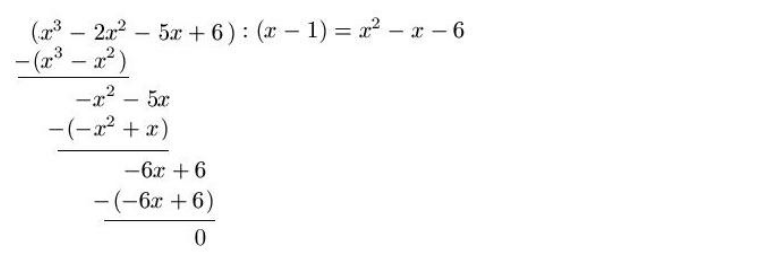
\includegraphics[width=0.7\linewidth]{img/polyDiv.png}\\
Andernfalls machen wir eine Partialbruchzerlegung:

\begin{align*}
	\frac{t+2}{t^2(t^2 + 2)} &= \frac{A}{t^2} + \frac{B}{t} + \frac{Ct + D}{t^2 + 2}\\
	\frac{t}{t^3 + t^2 - t - 1} &= \frac{A}{(t+1)} + \frac{B}{(t+1)^2} + \frac{C}{t-1} \quad \text{first polyDiv}\\
	\frac{t^4 + 1}{(t^2 + 1)^2} &= 1 + \frac{-2t}{(t^2 + 1)^2} = 1 + \ldots + \frac{At + B}{t^2 + 1} + \frac{Ct + D}{(t^2 + 1)^2}
\end{align*}


% -------------------------- Uneigentliche Integrale --------------------------

\section*{Uneigentliche Integrale}


Es gibt zwei Arten von uneigentlichen Integralen, man interessiert sich dafür ob die Integrale konvergieren oder nicht. Für beide Arten braucht man die gleichen Techniken:

\begin{enumerate}
	\item[] \textbf{Typ 1:} $f(x)$ auf $[a,\infty)$ stetig. Dann setzt man $\int_{a}^{\infty} f(x) dx = \lim_{R \to \infty} \int_{a}^{R} f(x) dx$ falls der Grenzwert existiert.
	\item[] \textbf{Typ 2:} $f(x)$ auf $(a,b]$ stetig. Dann setzt man $\int_{a}^{b} f(x) dx= \lim_{\epsilon \to 0^+} \int_{a+\epsilon}^{b} f(x) dx$ falls der Grenzwert existiert.
\end{enumerate}


\subsection*{Definition + direkte Berechung}
Setze die Definition ein (replace $\infty$ with $R$) und berechne dann das Integral. Lasse nun $R$ nach $\infty$ laufen.

\subsection*{Vergleichskriterium}
 Seien $f,g$ auf dem Integrationsgebiet stetig mit $0 \leq f(x) \leq g(x)$ für alle $x$. Dann gilt:
 \begin{enumerate}
 	\item Ist $\int_{a}^{\infty} g(x) dx$ konvergent, so auch $\int_{a}^{\infty} f(x) dx$
 	\item Ist $\int_{a}^{\infty} f(x) dx$ divergent, so auch $\int_{a}^{\infty} g(x) dx$
 \end{enumerate}
 Oft braucht man $\int_{1}^{\infty} \frac{1}{x^p} dx$ als Vergleichsmittel welches für $p>1$ konvergiert, für $p \leq 1$ ist es divergent.\\
\textbf{Beispiel (Vergleich)} 
\begin{itemize}
	\item $\int_{1}^{\infty} \frac{1 + e^x}{x} dx$, von unten durch $\int_{1}^{\infty} \frac{1}{x} dx$ abschätzen, dann divergent.
	\item $\int_1 ^\infty \sin^2\left(\frac{1}{x}\right) dx$, beachte dass wenn $x \geq 0$, $\sin(x) \leq x$ gilt. Somit haben wir Majorante $\int_{1}^{\infty} \frac{1}{x^2} dx$ und konvergent. 
\end{itemize}


\subsection*{Absolute Konvergenz}
$$ \int_{a}^{\infty} \left| f(x) \right| dx <\infty \implies \int_{a}^{\infty}f(x) dx < \infty $$
Das ist nützlich bei trigonometrischen Teilen.\\
\textbf{Beispiel (Absolute Konvergenz)} 
\begin{itemize}
	\item $\int_{1}^{\infty} \frac{\cos^2(x)}{x^2} dx$. Es gilt $\left| \frac{\cos^2(x)}{x^2}\right|\leq \frac{1}{x^2}$, somit konvergent.
	\item $\int_0 ^\infty x\sin(4x)e^{-2x} dx$. Es gilt $|x\sin(4x)e^{-2x}| \leq xe^{-2x}$ wenn $x\geq 0$, per partieller Integration konvergiert das zweite. Somit konvergent.
\end{itemize}

\subsection*{Mc. Laurin Konvergenzkriterium}
Sei $f:[1,\infty) \to [0,\infty)$ monoton fallend.
$$\sum_{n=1}^{\infty} f(n) \ \text{konv.}  \iff    \int_{1}^{\infty} f(x) dx \ \text{konv.}$$




% -------------------------- Gamma Funktion --------------------------

\section*{Gamma Funktion}

Die Gamma Funktion ist definiert als $\Gamma (s) := \int_{0} ^{\infty} e^{-x} x^{s-1} dx$.

Sie erfüllt:
\begin{itemize}
	\item $\Gamma(1) = 1$
	\item $\Gamma(s+1) = s\Gamma(s) \ \forall s > 0$
	\item $\Gamma$ ist logarithmisch konvex: $\Gamma(\lambda x + (1-\lambda)y) \leq \Gamma(x)^\lambda \Gamma(y)^{1-\lambda}$
\end{itemize}
Wir zeigen nun die zweite Eigenschaft mittels partieller Integration:
\begin{align*}
	\int_{0}^{b} x^n e^{-x} dx &= -b^n e^{-b} + n \int_{0}^{b} x^{n-1}e^{-x}
\end{align*}
Da $\lim_{b \to \infty}  -b^n e^{-b} = 0$ folgt: $\int_{0}^{\infty} x^n e^{-x} dx =n \int_{0}^{\infty} x^{n-1}e^{-x}$


% -------------------------- Sonstiges --------------------------









\section*{Sonstiges}
\begin{method}{Binomialsatz}
	$\forall x,y \in \mathbb{C}$, $n \geq 1$ gilt:
	$$(x+y)^n = \sum_{k=0}^{n} \binom{n}{k}x^k y^{n-k}$$
\end{method}

\begin{method}{ABC / Mitternachtsformel}
	\begin{align*}
		\text{Gegeben: } & ax^2 + bx + c = 0\\
		\text{Lösung: } & x_{1,2} = \frac{-b \pm \sqrt{b^2 -4ac}}{2a}
	\end{align*}
\end{method}


\begin{method}{Logarithmus Regeln}
${\displaystyle \log _{b}(x\cdot y)=\log _{b}(x)+\log _{b}(y)}$
\end{method}


\begin{method}{Summenformeln}
	\begin{align*}
	\sum _{{k=1}}^{n}k &= {\frac  {n(n+1)}{2}}\\
	\sum_{k=1}^n (2k-1) &= n^2\\
\sum _{{k=1}}^{n}k^{2} &= {\frac  {n(n+1)(2n+1)}{6}}
	\end{align*}
\end{method}


\begin{method}{Gerade \& Ungerade Funktion}
Eine Funktion heisst:
\begin{itemize}
	\item \textsc{Gerade} wenn $f(-x) = f(x)$
	\item \textsc{Ungerade} wenn $f(-x) = - f(x)$
\end{itemize}
Dabei sind $f(x) = 1$, $f(x) = |x|$, $f(x)=x^2$, $f(x) = \cos(x)$ alles gerade Funktionen.\\
Im Gegenzug sind $f(x) = sgn(x)$, $f(x) = x$, $f(x) = \tan(x)$, $f(x) = \sin(x)$ ungerade Funktionen.
\end{method}


\begin{method}{Injektiv}
	\begin{align*}
			&\forall x_1,x_2 \in M : f(x_1) = f(x_2) \implies x_1 = x_2\\
			\text{or }  &x_1 \not = x_2 \implies f(x_1) \not = f(x_2)
	\end{align*}
	\textbf{Surjektiv}
	\begin{align*}
	\forall y \in N \exists x \in M : y = f(x)
	\end{align*}
\end{method}

\textbf{Umkehrsatz - Beispiel} Zeige dass $x + e^x$ bijektiv von $\R$ auf $\R$ abbildet. Es gilt $f'(x) = 1 + e^x > 0$, somit ist $f$ streng monoton wachsend in $\R$ und Umkehrbar. Weil $\lim_{x \to -\infty} f(x) = - \infty$ und $\lim_{x \to \infty} f(x) = \infty$ ist $f$ bijektiv von $\R$ nach $\R$


\vfill\null
\columnbreak

% to have more vertical space in the table.

{\renewcommand{\arraystretch}{1.5}
	\begin{table}[]
		\begin{tabular}{@{} p{.25\textwidth} p{.3\textwidth} p{.45\textwidth} @{}}
			\toprule
			Funktion & Ableitung & Bemerkung / Regel\\ \midrule
			$x$ & $1$ &   \\
			$x^2$& $2x$ &   \\
			$x^n$& $n\cdot x^{n-1}$ & $n \in \R$  \\
			$\frac{1}{x} = x^{-1}$ & $- \frac{1}{x^2}$ & \\
			$\sqrt{x} = x^{\frac{1}{2}}$ & $\frac{1}{2\sqrt{x}}$ & \\ 
			$\sqrt[n]{x} = x^{\frac{1}{n}}$ & $\frac{x^{\frac{1}{n} -1 }}{n}$ &  $\int x^{1/n} dx = \frac{n x^{1/n + 1}}{n+1} + C$\\ 
			$e^x$ & $e^x$ & \\
			$a^x$ & $\ln(a) \cdot a^x$& \\
			$x^x = e^{x\log(x)}$ & $x^x \cdot (\log(x) + 1)$ & Kettenregel $e^{x\log(x)}$\\
			$\ln(x)$ & $\frac{1}{x}$ & \\
			$x\ln(x) - x$ & $\ln(x)$ &  \\ \midrule
			$\sin(x)$ & $\cos(x)$ & \\
			$\cos(x)$ & $- \sin(x)$ & \\ 
			$\tan(x) = \frac{\sin(x)}{\cos(x)}$ & $\frac{1}{\cos^2(x)} = 1 + \tan^2(x)$ &\\
			$\cot(x) = \frac{\cos(x)}{\sin(x)}$ & - $\frac{1}{\sin^2(x)}$ & \\ 
			$\arcsin(x)$ & $\frac{1}{\sqrt{1 - x^2}}$ & $ \arcsin : [-1,1] \to [-\frac{\pi}{2},\frac{\pi}{2}]$\\
			$\arccos(x)$ & $ - \frac{1}{\sqrt{1-x^2}}$ & $\arccos : [-1,1] \to [0, \pi]$\\
			$\arctan(x)$ & $\frac{1}{1+x^2}$ & $\arctan:(-\infty, \infty) \to (- \frac{\pi}{2},\frac{\pi}{2})$\\
			$\operatorname{arccot}(x)$ & $ - \frac{1}{1+x^2} $ & $\operatorname{arccot} : (-\infty, \infty) \to (0,\pi)$\\
			\midrule
			$\cosh(x)$ & $\sinh(x)$ &\\
			$\sinh(x)$ & $\cosh(x)$ & \\
			$\tanh(x)$ & $\frac{1}{\cosh^2(x)}$ & \\
			$\operatorname{arsinh}(x)$ & $\frac{1}{\sqrt{1+x^2}}$ & $\forall x \in R$\\
			$\operatorname{arcos}(x)$ & $\frac{1}{\sqrt{x^2 - 1}}$ & $\forall x \in (1, \infty)$\\		  $\operatorname{artanh}(x)$ & $\frac{1}{1-x^2}$ & $\forall x \in (-1,1)$\\
			\midrule
			$g(x) \cdot h(x)$ & $g(x) \cdot h'(x) + g'(x) \cdot h(x)$ & Produktregel\\
			$\left(g(x)\right)^n$ & $n \cdot \left( g(x) \right)^{n-1} \cdot g'(x)$ & Potenzregel\\
			$\frac{g(x)}{h(x)}$ & $\frac{ g'(x) \cdot h(x) - g(x)\cdot h'(x)}{\left(h(x)\right) ^2}$ & Quotientenregel\\
			$h(g(x))$ & $h'(g(x)) \cdot g'(x)$ & Kettenregel\\
			\bottomrule
		\end{tabular}
	\end{table}
}




\vfill\null
\columnbreak



\subsection*{Wichtige Integrale}

\begin{itemize}
	\item $\int \cos^2()x dx = \frac{\cos(x)\sin(x) + x}{2} + C$
	\item $\int \cos(x) \sin(x) dx = \frac{\sin^2(x)}{2}+C $
	\item $\int \sin^2(x) dx = \frac{x - \sin(x)\cos(x)}{2} + C$
	\item $\int \sqrt{1-x^2} dx = \frac{\arcsin(x) + x \sqrt{1-x^2}}{2} + C$
\end{itemize}



\newpage



\section*{First order differential Equations}



\begin{method}{Trennung der Variablen} Wenn wir eine ODE der Form $y' = h(x)y + b(x)$ haben so lösen wir das homogene Problem $y' = h(x)y$ mittels Trennung der Variablen.
	
Sei nun somit $y' = \frac{dy}{dx} = h(x)\cdot g(y)$ so schreiben wir es als 

\begin{align*}
	\frac{dy}{g(y)} &= h(x)dx\\
	\int \frac{dy}{g(y)} &= \int h(x)dx
\end{align*}
um, was wir dann nach $y$ auflösen können.
\end{method}


\TODO{beispiele}


\begin{method}{Variation der Konstanten} Wenn wir eine ODE der Form $y' = h(x)y + b(x)$ haben, so gilt dass $y(x) = y_{hom} + y_{part}$. Dafür lösen wir zuerst das homogene Problem mittels Trennung der Variablen.
	content...
\end{method}



\section*{Lineare DGL $n$-ter Ordnung}

Wir lösen das homogene Problem vor dem inhomogenen!

\begin{method}{Homogene Lineare DGL $n$-ter Ordnung}

Wenn wir eine Gleichung der Form
\begin{align*}
a_ny^{(n)} + a_{n-1}y^{(n-1)} + \ldots + a_0 y &= 0
\end{align*}
dann nehmen wir den Euler-Ansatz $y(x) = e^{\lambda x}$ und finden $\lambda$ mit
\begin{align*}
a_n \lambda^n + a_{n-1}\lambda^{n-1} + a_0 &= 0
\end{align*}
Nun finden wir die Nullstellen $\lambda$ des charakteristischen Polynoms. Wir bauen uns nun eine Basis aus $e^{\lambda_i x}$ Wenn eine Nullstelle $m$ mal Vorkommt nehmen wir
\begin{align*}
e^{\lambda x},e^{\lambda x}, \ldots , x^{m-1} e^{\lambda x} 
\end{align*}
Das gibt uns ein Fundamentalsystem. Die Allgemeine Lösung ist eine Linearkombination der Basis (basierend auf den Anfangswerten).
\end{method}

Wenn die NS $\lambda = \beta + i\gamma$ nicht reell ist, so ist (bei rellen DGL) auch $\beta -i\gamma$ auch eine NS. Wir konnen dann $e^{x(\beta + i\gamma)}$, $e^{x(\beta - i\gamma)}$ auswechseln durch $e^{x\beta}\cos(\gamma x)$ sowie $e^{x\beta}\cos(\gamma x)$ austauschen.



\TODO{beisiele}







\newpage

\section*{Continuity in $\R^n$}
\begin{method}{Convergence of sequence in $\R^n$}
	Let $(x_n)_n$ be a sequence  in $\R^n$. We say that a sequence converges to $y$ if for all $\epsilon > 0$, there exists $N \geq 1$ such that for all $n \geq N$ we have $\norm{x_n-y}\leq \epsilon$
\end{method}

\begin{method}{Continuity in $\R^n$}
	\begin{itemize}
		\item 	Let $x_0\in X$, we say that $f$ is continuous at $x_0$ if for all $\epsilon> 0$, there exists $\delta > 0$ such that if $x\in X$ satisfies $\norm{x-x_0}<\delta$ then $\norm{f(x) -f(x_0)}<\epsilon$.
		\item The function $f:X\to \R^m$ is continuous at $x_0$ if and only if, for every sequence $(x_n)_n$ in $X$ such that $x_k\to x_0$ as $k \to \infty$ the sequence $(f(x_k))_k$ converges to $f(x_0)$
	\end{itemize}
\end{method}

\section*{Differentiability in $\R^n$}

\subsection*{Rules for differentiation in $\R^n$}

\begin{method}{Gradient Vector}
	If $f:X\subseteq \R^n \to \R$ then we define $\nabla f(x_0)$:
	\begin{align*}
		\nabla f(x_0) &= 	\begin{pmatrix}
		\partial_{x_1} f(x_1)\\
		\ldots\\
		\partial_{x_n} f(x_0)
		\end{pmatrix}
	\end{align*}
\end{method}

\begin{method}{Jacobi Matrix}
	If $f(x) = (f_1(x),\ldots f_m(x))$ then we define
	\begin{align*}
		J_f(x) = \begin{pmatrix}
		\frac{\partial f_1}{\partial x_1}(x) & \ldots & \frac{\partial f_1}{\partial x_n}(x) \\
		\vdots & \ddots & \vdots \\
		\frac{\partial f_m}{\partial x_1}(x) & \ldots & \frac{\partial f_m}{\partial x_n}(x)	
		\end{pmatrix}
	\end{align*}
\end{method}

\begin{method}{Chain Rule}
	We have 
	\begin{align*}
		d(g \circ f)(x) = d(g(f(x)) = dg(f(x))\cdot df(x)
	\end{align*}
\end{method}
\textbf{Example}
\begin{itemize}
	\item Let $f(x,y,z)\mapsto (xy,y+z)$ and $g(x,y) \mapsto (e^x,xy)$.
	We have $dg(x,y) = \begin{bmatrix}
	e^x & 0 \\ y & x
	\end{bmatrix}$ as well as $df(x) = \begin{bmatrix}
	y & x & 0 \\ 0 & 1 & 1
	\end{bmatrix}$. From $dg$ we can find $dg(f) = \begin{bmatrix}
	e^{xy} & 0 \\ y+z & xy
	\end{bmatrix}$ This gives us for $d(g(f(x))) = dg(f(x))\cdot df(x)$:
	\begin{align*} \begin{bmatrix}
	e^{xy} & 0 \\ y+z & xy
	\end{bmatrix} \cdot \begin{bmatrix}
	y & x & 0 \\ 0 & 1 & 1
	\end{bmatrix} = 
	\begin{bmatrix}
	ye^{xy} & xe^{xy} & 0 \\ y^2+yz & 2xy +zx & xy
	\end{bmatrix}
	\end{align*}
	
	\item Let $f(x,y)\mapsto (e^x + \sin(xy), x+y^2x)$ and $g = f\circ f \circ f$. Find $dg(0,0)$: We have first notice that:
	\begin{align*}
		f(0,0) &= \begin{bmatrix}
		e^0 + \sin(0\cdot 0) & 0 + 0^2\cdot 0
		\end{bmatrix} = \begin{bmatrix}
		1 & 0
		\end{bmatrix}\\
		f(f(0,0)) &= f(1,0) = \begin{bmatrix}
		e^1 + \sin(1\cdot 0) & 1 + 0^2\cdot 1
		\end{bmatrix} = \begin{bmatrix}
		e & 1
		\end{bmatrix}
	\end{align*}
	Now we can use these results:
	\begin{align*}
		df(x,y) &= \begin{bmatrix}
		e^{x} + y\cos(xy) & x\cos(xy) \\1+y^2 & 2xy
		\end{bmatrix}\\
		df(0,0) &= \begin{bmatrix} 1 & 0 \\ 1 & 0
		\end{bmatrix}\\
		df(f(0,0)) &= df(1,0) = \begin{bmatrix}
		e & 1 \\ 1& 0
		\end{bmatrix}\\
		df(f(f(0,0))) &= df(e,1) =  \begin{bmatrix}
		e^e + \cos(e) & e\cos(e) \\ 2 & 2e
		\end{bmatrix}
	\end{align*}
	We can now insert these results: (calculating matrix product omitted)
	\begin{align*}
		dg(0,0) &= df(f(f(0,0)))\cdot df(f(0,0)) \cdot df(0,0) \\
		&= df(e,1) \cdot df(1,0)\cdot df(0,0)
	\end{align*}
\end{itemize}

\section*{Topology of $\R^n$}




\end{multicols}
\end{document}
